\documentclass[11pt,a4paper]{article}

\usepackage{style2017}
\usepackage{hyperref}

\hypersetup{
    colorlinks =false,
    linkcolor=blue,
   linkbordercolor = 1 0 0
}
\newcounter{numexo}
\setcellgapes{1pt}

\definecolor{codegreen}{rgb}{0,0.5,0}
\definecolor{codeblue}{rgb}{0,0.1,0.6}
\definecolor{codegray}{rgb}{0.5,0.5,0.5}
\definecolor{codepurple}{rgb}{0.5,0,0.8}
\definecolor{codered}{rgb}{0.9,0.1,0.1}
\definecolor{backcolour}{rgb}{0.95,0.95,0.92}
\lstset{
	language=python,
	%frame=single,
	xleftmargin=3em,
	xrightmargin=2em,
	%backgroundcolor=\color{backcolour},   
    commentstyle=\color{codegreen},
    keywordstyle=\color{codepurple},
    numberstyle=\color{black!80!white},
    stringstyle=\color{codered},
    basicstyle=\ttfamily,
    %columns=[l]flexible,
    breakatwhitespace=false,         
    breaklines=true,                 
    captionpos=b,                    
    keepspaces=true,                 
    %numbers=none,                    
    %numbersep=1em,               
    showspaces=false,                
    showstringspaces=false,
    showtabs=false,                  
    tabsize=2,
    emph={False,True,self},
    emphstyle=\color{codeblue}
}

\lstset{%
	inputencoding=utf8,
	extendedchars=true,
    literate=%
    {é}{{\'e}}{1}%
    {è}{{\`e}}{1}%
    {à}{{\`a}}{1}%
    {ç}{{\c{c}}}{1}%
    {œ}{{\oe}}{1}%
    {ù}{{\`u}}{1}%
    {É}{{\'E}}{1}%
    {È}{{\`E}}{1}%
    {À}{{\`A}}{1}%
    {Ç}{{\c{C}}}{1}%
    {Œ}{{\OE}}{1}%
    {Ê}{{\^E}}{1}%
    {ê}{{\^e}}{1}%
    {î}{{\^i}}{1}%
    {ô}{{\^o}}{1}%
    {û}{{\^u}}{1}%
    {ë}{{\¨{e}}}1
    {û}{{\^{u}}}1
    {â}{{\^{a}}}1
    {Â}{{\^{A}}}1
    {Î}{{\^{I}}}1
}
    
\begin{document}


\begin{NSI}
{Exercice}{Dictionnaire en Python}
\end{NSI}


\addtocounter{numexo}{1}
\subsection*{\Large Exercice \thenumexo}
On donne le dictionnaire suivant:

\begin{lstlisting}
animaux={
	'chien':'rouky',\
	'chat':'berlioz',\
	'éléphant':'dumbo',\
	'ours':'baloo',\
	'panthère': 'bagheera',\
	'serpent':'kaa',\
	'renard':'rox'
}
\end{lstlisting}

\begin{enumerate}
\item Est-il possible d'ajouter la clef \textsf{tigre} avec la valeur \textsf{shere khan} au dictionnaire? Justifier.
\item Est-il possible d'ajouter la clef \textsf{chien} avec la valeur \textsf{pongo} au dictionnaire? Justifier.
\item Comment récupérer la valeur \textsf{berlioz} de ce dictionnaire ?
\item Comment récupérer la valeur de la clef \textsf{panthère} du dictionnaire?
\item Comment ajouter la souris nommée \textsf{bernard} au dictionnaire ?
\item Comment ajouter aussi la souris nommée \textsf{Bianca} au dictionnaire ?
\item Comment remplacer la clef \textsf{serpent} par la clef \textsf{snake} en gardant la valeur \textsf{kaa}?
\item Comment récupérer dans une liste python toutes les clefs du dictionnaire ?
\item Comment récupérer dans une liste python toutes les valeurs du dictionnaire ?
\item Comment connaitre le nombre d'éléments de ce dictionnaire ?
\end{enumerate}

\addtocounter{numexo}{1}
\subsection*{\Large Exercice \thenumexo}
On considère un dictionnaire \textbf{notes} qui a la structure suivante:
\begin{itemize}[label=\textbullet]
\item Les clés sont des matières (maths, français,...);
\item Les valeurs sont des moyennes de type entier.
\end{itemize}
Par exemple:
\begin{lstlisting}
notes={'maths':12,'francais':11,'nsi':14,'anglais':13,'eps':10}
\end{lstlisting}
\begin{enumerate}
\item Écrire une fonction \textsf{ajouter\_note} qui a pour paramètres un dictionnaire, une matière et une note. Cette fonction renvoie le dictionnaire en ajoutant à celui-ci la matière et la note . Si la matière est déjà présente dans le dictionnaire, seule la note est modifiée.

\item Écrire une fonction \textsf{modifier\_note} qui a pour paramètres un dictionnaire, une matière et une note. Cette fonction  renvoie le dictionnaire avec la note modifiée.

\item Écrire une fonction \textsf{supprimer\_note} qui a pour paramètre un dictionnaire Cette fonction renvoie le dictionnaire en supprimant la matière (et la note associée) passée en argument.

\item Écrire une fonction \textsf{calculer\_moyenne} qui a pour paramètre un dictionnaire et qui calcule la moyenne des notes du dictionnaire.

\item Écrire la fonction \textsf{min\_et\_max} qui prend en argument un dictionnaire et renvoie un dictionnaire contenant la matière et la note minimale ainsi que la matière et la note maximale. 

En cas de doublon, ceux-ci devront apparaître dans le dictionnaire.

\item Tester vos fonctions :
\begin{enumerate}
\item Ajouter la matière \textsf{espagnol} et la note $17$.
\item Modifier la note de \textsf{nsi} avec la valeur $15$.
\item Supprimer la note de la matière \textsf{eps}.
\item Calculer la moyenne des notes.
\item Afficher le dictionnaire contenant la note minimale et la note maximale.
\end{enumerate}
\end{enumerate}


%\addtocounter{numexo}{1}
%\subsection*{\Large Exercice \thenumexo}
%On va créer un dictionnaire pour afficher une fiche identité de célébrités.
%\begin{enumerate}
%\item Créer un dictionnaire \textbf{célébrités} ayant la structure suivante :
%\begin{itemize}
%\item Les clés du dictionnaire sont des personnalités célèbres (noms);
%\item Les valeurs sont des tableaux contenant dans l'ordre : la nationalité, l'année de naissance, l'année de décès et leur activité professionnelle. 
%\end{itemize}
%Par exemple : \textbf{zidane} est la clé pour les valeurs ['france','1972','',football']
%\item Créer plusieurs entrées dans votre dictionnaire au moins trois.
%\item Créer une fonction \textbf{saisir} qui permet d'ajouter des célébrités à votre dictionnaire en saisissant les valeurs dans des \textbf{input} (voir ci-dessous).
%\begin{center}
%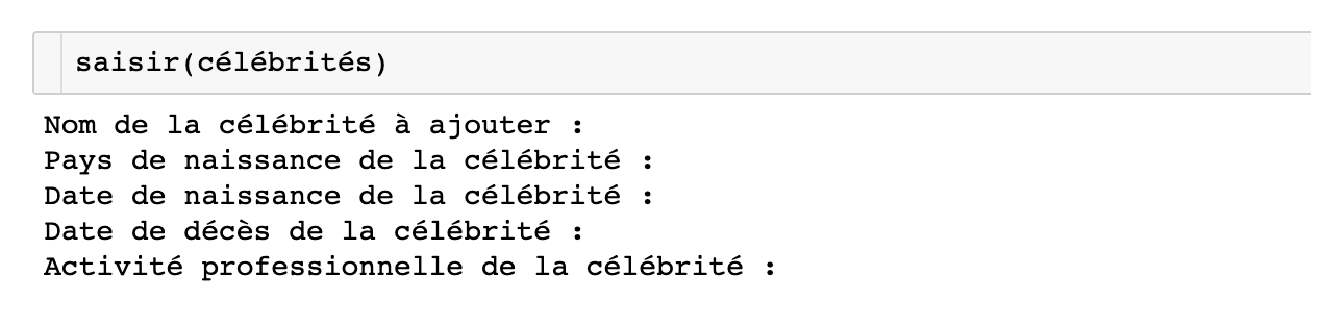
\includegraphics[scale=0.6]{img/celebrite1.eps}
%\end{center}
%Saisissez avec votre fonction 3 nouvelles célébrités et vérifiez que le dictionnaire est bien structuré.
%\begin{center}
%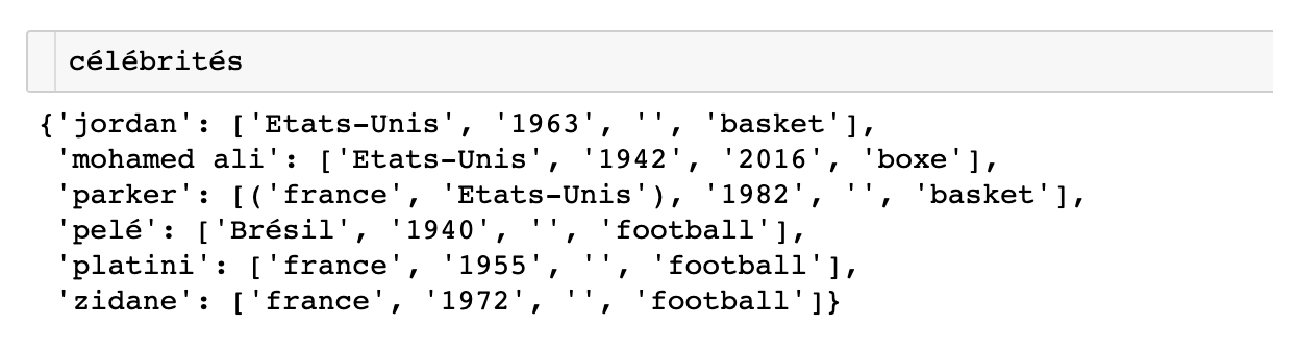
\includegraphics[scale=0.6]{img/celebrite2.eps}
%\end{center}
%\item Créer une fonction \textbf{pays} qui prend en paramètre le dictionnaire et une clé du dictionnaire et retourne le pays d'origine de la célébrité (voir ci-dessous).
%\begin{center}
%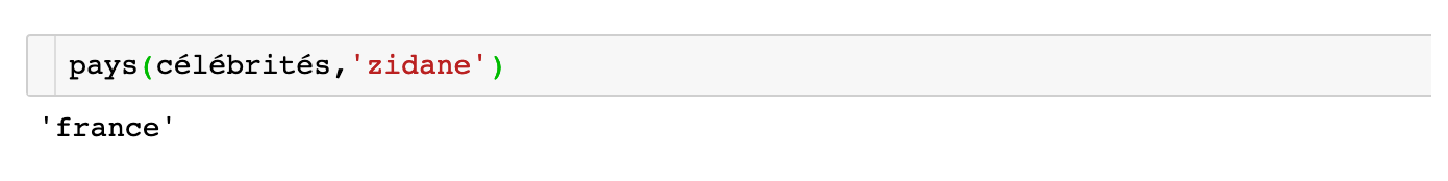
\includegraphics[scale=0.55]{img/celebrite3.eps}
%\end{center}
%\item Créer de même la fonction \textbf{naissance} qui retourne l'année de naissance de la célébrité.
%\item Créer de même une fonction \textbf{vivant} qui retourne une valeur booléenne (True, False) et vérifie si la célébrité est toujours vivante.
%\begin{center}
%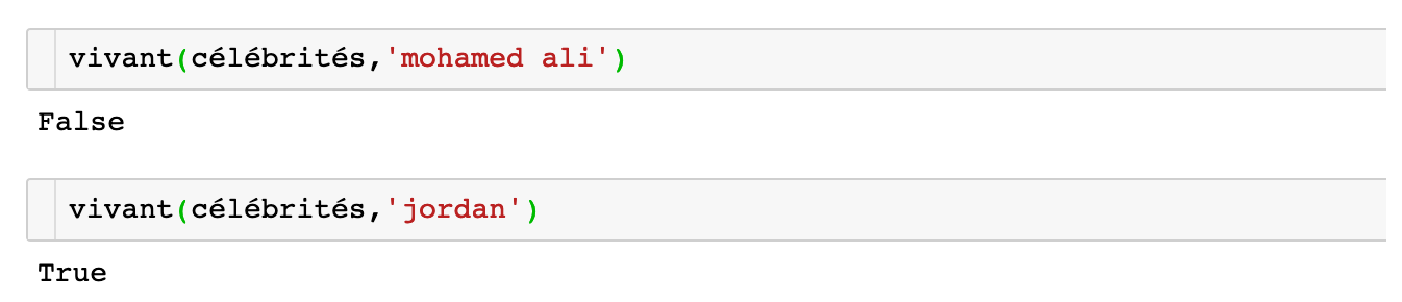
\includegraphics[scale=0.55]{img/celebrite4.eps}
%\end{center}
%\item Écrire une fonction \textbf{age} qui donne l'âge de la célébrité. Attention, les années saisies sont des chaines de caractères, donc pour effectuer les calculs, il faut les convertir en "integer" avec la fonction \textbf{eval}.
%\item Créer la fonction \textbf{activité} qui retourne l'activité de la célébrité.
%\item Écrire une fonction \textbf{cle\_de\_valeur} qui liste toutes les célébrités (clés) qui ont une valeur commune. Par exemple, la même nationalité, la même année de naissance ou la même activité.
%\begin{center}
%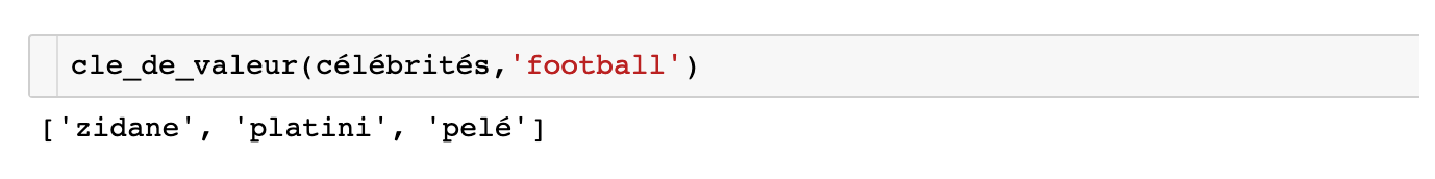
\includegraphics[scale=0.55]{img/celebrite5.eps}
%\end{center}
%\item Créer une fonction \textbf{identité} qui liste toutes les informations sur la célébrité se trouvant dans le dictionnaire. La fonction retournera un texte sur plusieurs lignes.
%\begin{center}
%\includegraphics[scale=0.5]{img/celebrite6.eps}
%\end{center}
%\item Pour finir, écrire un programme qui prend en saisie une valeur à chercher dans le dictionnaire et qui affiche toutes les valeurs (ou clés) trouvées en concordance.
%\begin{center}
%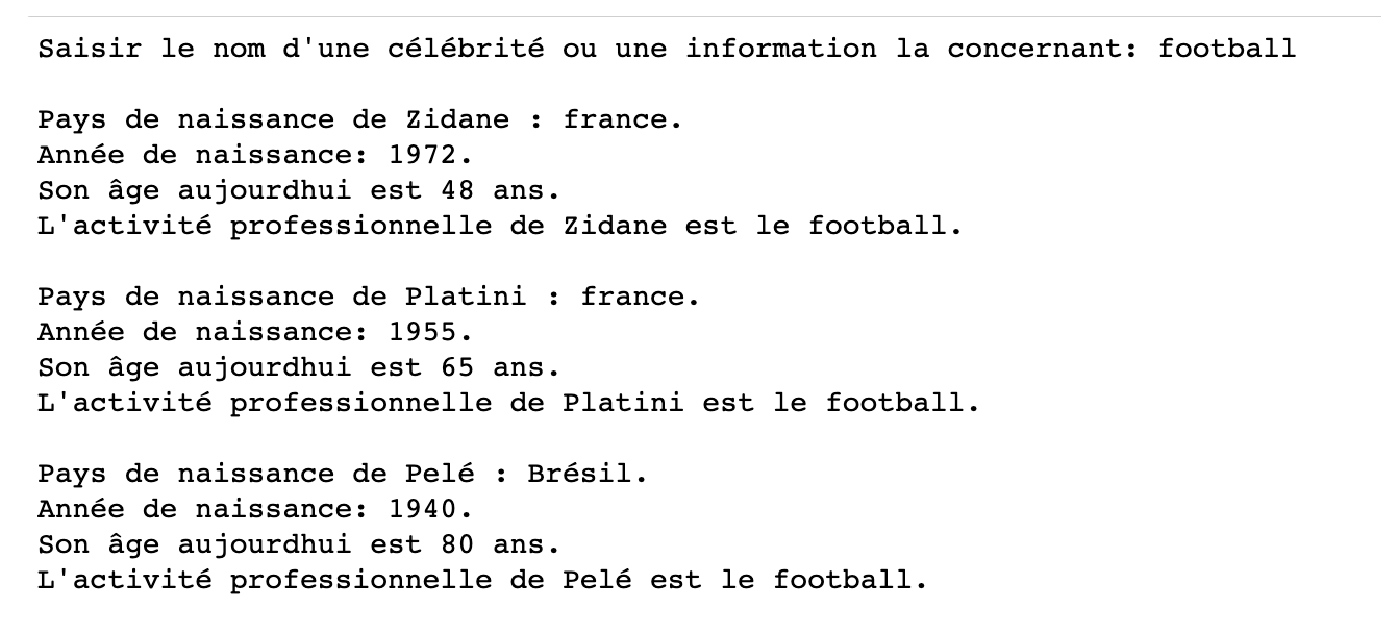
\includegraphics[scale=0.6]{img/celebrite7.eps}
%\end{center}
%\item Pour aller plus loin, on traitera aussi les cas ou rien n'est trouvé et également en prenant compte de la syntaxe utilisée (majuscules ou non).
%\item Améliorer le code pour gérer les éventuelles erreurs dues à une mauvaise saisie.
%\end{enumerate}

\addtocounter{numexo}{1}
\subsection*{\Large Exercice \thenumexo }

On dispose de \textbf{fiches} de renseignements sur des individus contenant leur nom, leur couleur préférée et l'instrument de musique qu'il joue. L'objectif est de réaliser des recherches par critères : nom, couleur ou instrument.

On commence par créer des fiches aléatoires puis on écrira notre fonction de recherche.

\begin{enumerate}
\item Créer les listes suivantes (vous pouvez modifier ou ajouter des valeurs à ces listes) :

\begin{center}
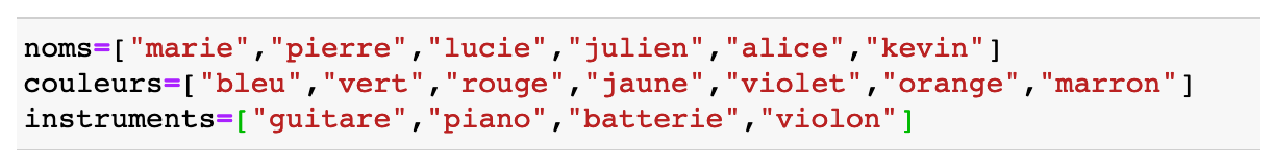
\includegraphics[scale=0.6]{img/dicoliste1.eps}
\end{center}

\item Écrire une fonction \textsf{aleadico} qui a 3 paramètres \textsf{n}, \textsf{c} et \textsf{i} correspondant aux listes \textsf{noms}, \textsf{couleurs} et \textsf{instruments}.

Cette fonction renvoie un dictionnaire dont les clés sont \textsf{nom}, \textsf{couleur} et \textsf{instrument} et dont les valeurs sont choisies aléatoirement parmi les trois listes \textsf{noms}, \textsf{couleurs} et \textsf{instruments}.

Ci-dessous un exemple de dictionnaire renvoyé par la fonction.

\begin{center}
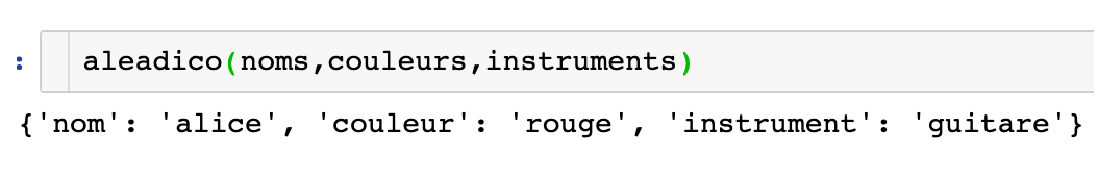
\includegraphics[scale=0.6]{img/dicoliste2.eps}
\end{center}

\item Écrire un code en Python qui crée le tableau (liste) \textsf{fiches} contenant 20 dictionnaires créés par la fonction \textsf{aleadico}. 
%\begin{center}
%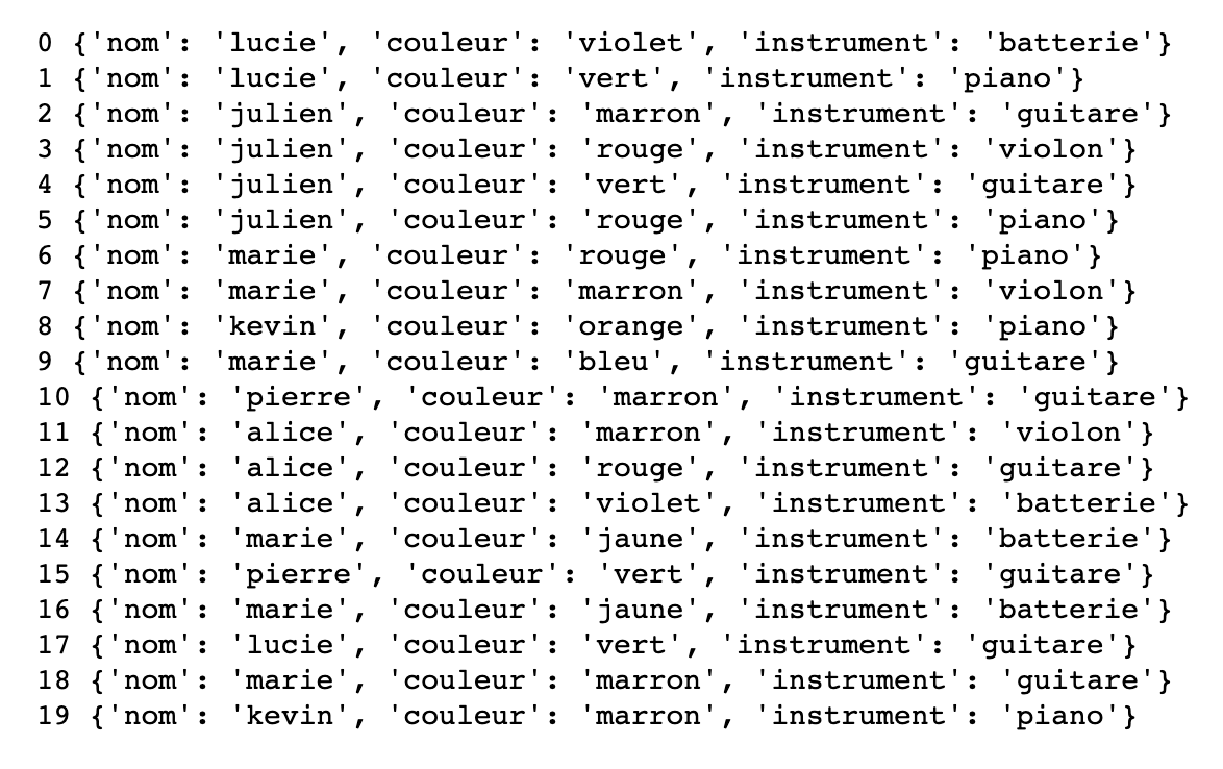
\includegraphics[scale=0.6]{img/dicoliste3.eps}
%\end{center}

\item Écrire une fonction \textsf{recherche\_nom} qui a pour paramètre \textsf{nom} de type chaine de caractères. 

Cette fonction renvoie la liste des dictionnaires qui ont comme valeur de nom le nom passé en argument. S'il n'y aucune valeur correspondante, la fonction renvoie une liste vide.

\item Modifier la fonction précédente pour effectuer une recherche aussi sur la couleur et l'instrument de musique. 

La fonction renvoie une liste de dictionnaires contenant la valeur passée en paramètre.

\item Effectuer les recherches suivantes:
\begin{enumerate}
\item Rechercher les fiches ayant le nom \textsf{lucie}.
\item Rechercher les fiches ayant la couleur \textsf{bleu}.
\item Rechercher les fiches ayant l'instrument \textsf{guitare}.
\item Créer une liste qui contient les fiches ayant le nom \textsf{lucie} ou la couleur \textsf{bleu}.
\item Créer une liste qui contient les fiches ayant le nom \textsf{lucie} et l'instrument \textsf{guitare}.
\end{enumerate}

\textbf{Remarque:} si votre dernière recherche est vide, il est possible qu'il n'y ait pas de fiche correspondante. Dans ce cas, ajouter une fiche pour avoir un retour non vide.
\end{enumerate}


\end{document}
